%%%%%%%%%%%%%%%%%%%%%%%%%%%%%%%%%%%%%%%%%%%%%%%%%%%%%%%%%%%%%%%%%%%%%%%
%% Main Document
%%%%%%%%%%%%%%%%%%%%%%%%%%%%%%%%%%%%%%%%%%%%%%%%%%%%%%%%%%%%%%%%%%%%%%
\documentclass[a4paper,11pt]{article}

% General  instructions / Best Practice Rules:
% ------------------------------------
% * Only one sentence per line!
% * Use active voice whenever possible! ("we have investigated" instead of "it
%   was investigated")
% * Use past progressive instead of simple past! ("Banks et al. have shown"
%   instead of "Banks et al. showed")
% * Mark open points with \todo{ <Name of assigned person>: ... }
% * Only commit after checking that it compiles. 
% * Use \cref{<label>} only, no \ref !
% * For abbreviations, always use the Glossaries package and \gls{<abbrv>} or
%   \glspl{<abbrv>} ! --> ensures that every abbreviation is introduced correctly


%%%%%%%%%%%%%%%%%%%%%%%%%%%%%%%%%%%%%%%%%%%%%%%%%%%%%%%%%%%%%%%%%%%%%%%
%% EIT Package and Language Settings
%%%%%%%%%%%%%%%%%%%%%%%%%%%%%%%%%%%%%%%%%%%%%%%%%%%%%%%%%%%%%%%%%%%%%%

% document with serif font
% use [de] option for German documents
%\usepackage{style-eit-latex/EIT}
%\usepackage[de]{style-eit-latex/EIT}

% use [pt] option for PT Sans without serif
\usepackage[pt]{style-eit-latex/EIT}
%\usepackage[pt, de]{style-eit-latex/EIT}


%%%%%%%%%%%%%%%%%%%%%%%%%%%%%%%%%%%%%%%%%%%%%%%%%%%%%%%%%%%%%%%%%%%%%%%
%% Custom Packages
%%%%%%%%%%%%%%%%%%%%%%%%%%%%%%%%%%%%%%%%%%%%%%%%%%%%%%%%%%%%%%%%%%%%%%
\usepackage[]{algorithm2e}
\usepackage{algorithmicx}
\usepackage{algpseudocode}

\algdef{SE}[DOWHILE]{Do}{doWhile}{\algorithmicdo}[1]{\algorithmicwhile\ #1}%
% TODO: add own packages here


%%%%%%%%%%%%%%%%%%%%%%%%%%%%%%%%%%%%%%%%%%%%%%%%%%%%%%%%%%%%%%%%%%%%%%%
%% Hyphenation
%%%%%%%%%%%%%%%%%%%%%%%%%%%%%%%%%%%%%%%%%%%%%%%%%%%%%%%%%%%%%%%%%%%%%%

% correct bad hyphenation here
\hyphenation{net-works semi-conduc-tor quad-ra-ture mat-ches trans-form meth-od}


%%%%%%%%%%%%%%%%%%%%%%%%%%%%%%%%%%%%%%%%%%%%%%%%%%%%%%%%%%%%%%%%%%%%%%%
%% Document Configuration
%%%%%%%%%%%%%%%%%%%%%%%%%%%%%%%%%%%%%%%%%%%%%%%%%%%%%%%%%%%%%%%%%%%%%%
% import global settings file
\input{includes/settings}

% TODO: add own settings here


%%%%%%%%%%%%%%%%%%%%%%%%%%%%%%%%%%%%%%%%%%%%%%%%%%%%%%%%%%%%%%%%%%%%%%%
%% Title and Document Information
%%%%%%%%%%%%%%%%%%%%%%%%%%%%%%%%%%%%%%%%%%%%%%%%%%%%%%%%%%%%%%%%%%%%%%

\begin{document}

% Title, author and other information:
\title{Formal Verification in the context of Highly Configurable IPs}
\subtitle{Master thesis to obtain : European Master in Embedded Computing Systems}
\author{Sebastian Lee Barrera}

\maketitle


%%%%%%%%%%%%%%%%%%%%%%%%%%%%%%%%%%%%%%%%%%%%%%%%%%%%%%%%%%%%%%%%%%%%%%%
%% Body Text
%%%%%%%%%%%%%%%%%%%%%%%%%%%%%%%%%%%%%%%%%%%%%%%%%%%%%%%%%%%%%%%%%%%%%%

% INSERT YOUR CONTENT HERE:
%

\section{Introduction}
The ever growing microelectronics and semi-conductor industry demand for novel  techniques on design and verification in order to meet aggressive and tight schedules as well as to cope with today's big design sizes.
Verification has always played a key role in the design cycle, as much as important as time consuming. Recent studies show that verification consumes around half of the time of the whole design cycle. In this matter, formal methods have experienced a considerable increase on their adoption on industry as a result of mature algorithms and tools. Nevertheless, there still exists the question of how much of the traditional simulation-based verification can be relieved by formal methods and how to apply effectively formal tools. In addition to this problems, the great degree of automation present on highly configurable IPs, adds an extra layer of complexity to the application of formal methods on industrial-scale designs. In this thesis a "Formal First" approach is explored in the context of highly configurable IPs.Two exemplary industrial IPs are analyzed under this flow. On the first half of the thesis, a method is proposed to cope with the high level of configurability of todays IPs and the subsequent application of formal methods is evaluated and analyzed. On the second half, we analyze the application of formal first approach on a high control based structure, we compare the existing verification plan and compare with the application of formal against the traditional simulation based activities. 
\subsection{Motivation}
A recent study \cite{mentor:study} from 2016 in Design and Verification trends from a lead EDA company, shows that around 50\% of designs re-spins are caused by functional or logical errors. This results show that, in spite of novel verification techniques and methodologies and standards, this has only been enough to cope with the constant increase of the design size in the recent years. The adoption of Automatic Formal Verification tools experienced a 62\% percent between 2012 and 2014, this shows the increasing interest from industry in formal verification as an effort to aid into the traditional verification flow. Specifically, formal property verification experienced a 31\% growth on its adoption in industry. This data shows a clear shift in industry to formal methods to aid with the big verification challenges on todays designs. The new challenge is how to apply this promising novel verification tools in industrial designs effectively and efficiently.

\subsection{Thesis structure}
This work presents first the concept of design verification on digital systems, starting from the current simulation based approach that is widely adopted in todays industry flows and paving the way to the need of formal methods. Afterwards, a brief theory on the principles of operation of formal property checking is discussed, particularly the essentials of Bounded Model Checking and Interval Property Checking are covered. A detailed and comprehensive description of the principles and theory behind state-of-the-art formal verification tools is beyond of the scope of this work. Nonetheless the theory discussed should be enough to grasp the general principle of operation and how we can use formal tools in a efficient way. 
Posterior to the theory discussion, two case studies are presented, both industrial highly configurable IP designs. The first design consists of a high portion of combinational logic and a relatively low register count, making it suitable to explore the application of formal verification. In this case study, a proposed flow is applied to cope with the high configurability of the design. The implemented flow is compared to the traditional planned simulation based approach. The second IP consists of a heavy control based structure, consisting of Finite State Machines (FSM) and combinational logic. In this example, the applied flow is analyzed and compared against its simulation counterpart. An analysis of the traditional activities, their time estimation and their findings is realized in comparison to the application of formal as a first verification approach.
\pagebreak
\section{A brief history of verification}
\subsection{Digital design verification: A brief overview}
Typically a design flow consists in a series of a consecutive steps of refinement. Normally the design starts with a high level specification of the desired functionallity that consists on a algorithmic or functional specification. This specification can be a plain document or a model in a high level language such as SystemC or C++. This specification is then refined, an architectural model is then created. Different types of implementations are analyzed and their trade-offs evaluated. After a detailed analys, an architecture is chosen to be implemented according to timing, area and other constraints, which is in, in a typical flow, described via means of a Hardware Description Language (HDL) at the Register Transfer Level (RTL). Every refinement step is error prone, and therefore, requires a corresponding verification step to ensure that the refinement still fulfills the specification and performs the desired functionality.Fig. 1 shows this refinement and abstraction relationship. 
\begin{figure}[h]
\centering
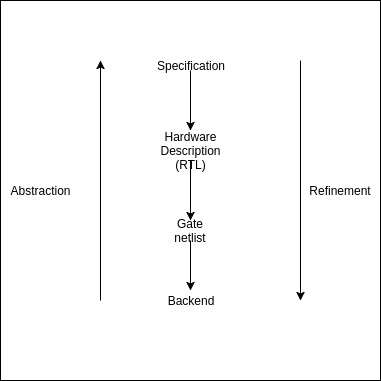
\includegraphics[width=0.4\textwidth]{design_flow.jpg}
\caption{Typicall Design Flow}
\end{figure} 
We focus on a specific verification step, functional verification, which ensures the corresponding RTL description implements the described architecture. To this end, the purpose of verification is more than "finding bugs", it should be prove extensively and comprehensively that the implementation meets the specification. The verification engineer typically creates a reference model to what his or her interpretation is of the specification is. This process adds implicitly redudancy to the design process\cite{sv_verif:sv}. In \cite{ovm_cb} is pointed out that the verification process involves two main questions:
\begin{itemize}
\item Does it work?
\item Are we done?
\end{itemize}
The first question relates to the functional correctness of the design under verification (DUV). Functional correctness proves that the design response is the expected under certain specific situations. The response of the DUV is compared to a reference model to check whether it meets the specification or not. 
\begin{figure}[h]
\centering
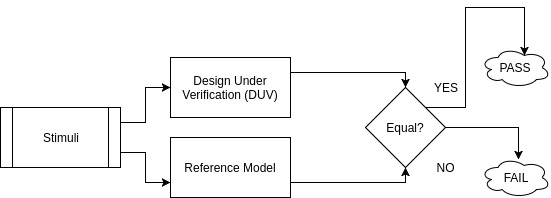
\includegraphics[width=0.7\textwidth]{doesitwork.jpg}
\caption{Doest it work? Flowchart}
\end{figure} 
Are we done question tries to address the problem of if we have sufficiently verified the design. Have we written enough tests or assertions? What are the use-cases we must ensure the design performs accordingly? Have we tested certain corner-cases that are expected to happen in the real environment? In order to address this questions we must first need what exactly is expected to be verified. 
This is captured typically on a Verification Plan. The Verification Plan describes the intended functionality to be tested, contains the metrics that are expected to be covered by the verification process and the means to achieve it. 
Complete frameworks and methodogies to address this two questions exists. 
Verification methodologies can be grouped into two main categories:
\begin{itemize}
\item Dynamic verification
\item Static  verification
\end{itemize}
We will describer briefly both approaches, pointing out the advantages and limitations of both, paving the way to the Formal First approach we propoose. 
\subsection{Dynamic Verification}
On the dynamic verification approach main focus relies on how to generate significant stimulus to take the DUV to a interesting state. The most basic approach for this is called "Directed testing", which consists on specifying all the desired inputs at all interesting points in time. In old times, plain text files containing stimulus/expected-response pairs where fed into the test-bench. The clear limitation of this approach was only testing specific sections of the design space. With the increasing size of designs, the need for more sofisticated verification techiniques became evident and novel and interesting methodologies were developed. This methodologies where based in the following principles:
\begin{itemize}
\item Layered Test-bench structure
\item Constrained Random Stimulus (CRS)
\item Maximum re-usability and configurability
\item Functional Coverage
\end{itemize}
%\bibliographystyle{plain}
%\bibliography{<path to your bibliography>}
This principles are closely realated to each other. As design grew in size and complexity so did the test-bench structure needed to test them. A layered test-bench structure aids this situation by breaking the problem into smaller pieces that are easier to develop and mantain. By allowing the stimulus to be random (CRS) 
, input vectors are generated automatically and can exercise areas of the design where issues where not expected. By constraining the input stimuli we mimic the real-wolrd environment the design is expected to operate in. Letting the stimulus to be generated automatically creates the problem of measuring how many interesting areas of the design have been already tested. How many are left? How much progress have done? To address this questions the concept of functional coverage was developed. Each item on the verification plan is then mapped to a so-called functional cover-point. Modern Electronic Design Automation (EDA) tools can keep score of which coverage points are being hit with each semi-random test, therefore the quality of a test can be measured by the coverage it provdes. Functional coverage provides a metric to measure the progress of the verification activity over time. Traditional HDLs were not sufficient to provide re-usability and configurability to verification infrastucture, new specialized were developed such as Specman and Vera. The current trend \cite{mentor:study} is to adopt SystemVerilog as an unified language for HDL, test-bench development and formal property development. SystemVerilog provies Object Oriented Programming (OOP) like features such as inheritance, classes, encapsulation, etc. This characteristics provide means to create highly re-usable and configurable verification environments but even with an unified language verification lacked a unified methodology that collected all the best practices and provided a common framework. Accellera Systems Initiative is an independent organization that supports and develops of, among many others, verification standards. One of the most widely adopted standards is the Universal Verification Methodology (UVM), partially based on Open Verification Metholodogy (OVM). Fig.3 shows a simplification of the UVM basic verification environment:
\begin{figure}[h]
\centering
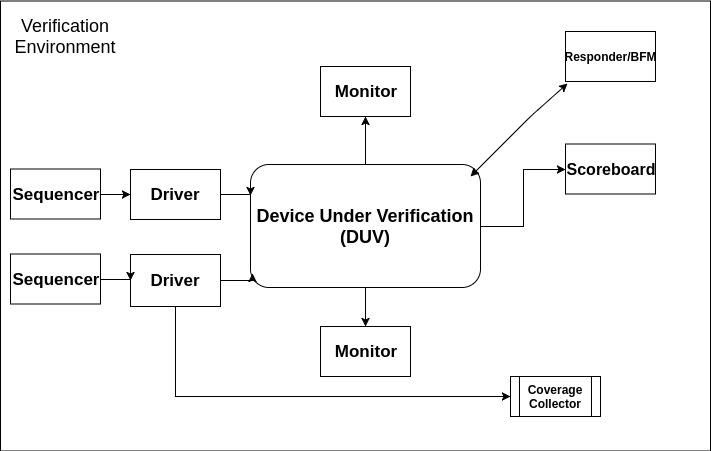
\includegraphics[width=0.7\textwidth]{uvm_environment.jpg}
\caption{Simplified verification environment}
\end{figure} 
This methodology effectively turns plain simulation into verification, enabling re-usability between components and providing an infrastucture to verify complex designs. Describing the Universal Verification Metholody comprehensively is beyond the scope of this thesis, nevertheless we will provide a brief description of the basic verification components:
\begin{itemize}
\item Sequencer: Generates chunks of data at a high abstraction level, typically at at the level of transaction. 
\item Driver: Is responsible of generating the pin level activity corresponding to a transaction generated by the sequencer. 
\item Monitor : Collects information about the traffic coming in and from the DUV.
\item Scoreboard :  Checks the response of the DUV and determines if it matches with the expected response.
\item Coverage collector: Keeps track of the functional coverage goals hit by the current stimuli.
\item Responder : Usually called Bus Functional Model (BFM), is a model of the connected blocks that mimics their behavior when the DUV interacts with them.
\end{itemize}
At this point is important to mention that an IP can be verified at various levels depending of the level of integration with other components. Naming of this levels differs between companies but the main verification levels are usually:
\begin{itemize}
\item IP or Block level: tests functionality of a single design block. Bus Functional Models are nromally used to mimic the parts that interact with it.
\item Cluster level : A collection of blocks that work closely together, such as a Memory Subsystem. 
\item System On Chip (SoC) or Full Chip (FC) level: Normally the highest level of integration containing all the design blocks.
\end{itemize}
As we go higher on the verification level, simulation speed is greatly reduced. Therefore, exhaustive testing should be tested at lower levels, leaving only interface and use-case testing to Cluster and SoC verification activities. 
Up to this point we have described how the problem of generating significant stimulus has been reliefed partially by novel methodologies and Hardware Verification Languages. Generating all possible stimulus is in most practical cases virtually impossible. Consider a 32-bit adder, consisting of two 32-bit wide inputs. To verify every single possible input we would need:
\begin{equation}
\#input\_vectors = (2^{32}) * (2^{32}) = 1.84 x 10^{19}
\end{equation} 
Exercising all this input vectors becomes unpractial as design sizes become bigger. 
\pagebreak
\subsection{A briefer history of Formal Verification}
The dynamic verification approach has a so-called Deep-first nature. It seeks to put the system on a specific state and check its response by predicting it. The disadvantage of this method is that it can only verify if the output is correct for a given stimuli. In formal verification this mindset is reversed, the verification engineer starts by specifying the desired behavior in a formal language and lets the formal checker prove or disproves it. The user is not concerned with the way the stimuli is generated at all. Formal verification therefore adopts a Breadth-first approach, that is, it checks if the output is valid for all possible input vectors. 
\begin{figure}[h]
\centering
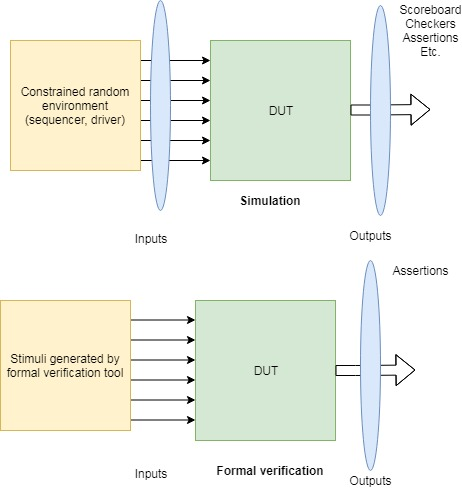
\includegraphics[width=0.7\textwidth]{formal_diagram.jpg}
\caption{Two different approaches: Formal and Simulation based verifiation}
\end{figure} 
Formal verification, rigurously speaking is defined as the act of proving or disproving the correctness of intended algorithms underlying a system with respect to a certain formal specification, using formal methods of mathematics\cite{whatisformal:EE}. There are two important aspects of formal verification:
\begin{itemize}
\item Equivalence checking
\item Model checking : Formal property verification
\end{itemize}
Equivalence checking is an important part of formal verification that deals with the problem of proving or disproving if two circuits are functionally equivalent. This is specially used to prove if netlists implementations of RTL descriptions are consistent.
On the other hand, model checking, the main subject of formal verification, has the goal to prove or disprove that a circuit posseses a property part of a specification. Formally, model checking refers to the problem of, given a model of a system, exhaustively and automatically check whether this model meets a given specification \cite{clarke:birth_model_checking}. We can note from this definition that, in oder to verify formally a circuit, we need three basic components:
\begin{itemize}
\item A model to describe matematically or formally the circuit to be verified.
\item A language to describe the specification this cirucuit is supposed to meet in a formal way.
\item An algorithm to prove exhaustively and conclusively if the model meets the specification under any possible valid condition.
\end{itemize}
A property about a design describes in a formal way a part of the functionality that a design must hold or avoid. We will describe three approaches to property checking: first we will describe algorithms that rely on graph-based algorithms, then we will cover bounded model checking basics, interval property checking and finally their relation with state-of-the-art model checking tools. 
\subsection{Temporal Structure and Computation Tree}
One approach to formal property checking is model checking using computation tree. The matematical model used to represent the circuit is called a Kripke Structure, which is basically a state diagram without inputs and outputs and its transition function depends only on the present state. Matematically a Kripke structure is defined as 4-tuple:
\begin{equation}
K = ( S , S_0 , T , A , L )
\end{equation}  
Where S represent the set of states, S$_0$ the set of initial states , T is the transition relation that maps a present state to a next one, A consists of a set of atomic formulas that can be true or false and L is a labeling function to link each state with propositional variables that are held true on it. By unrolling a Kripke structure we can trace out all paths from the initial states, if it contains loops this paths will be infinite, resulting in a tree structure. Figx ilustrates this concept :
The language used on this approach is called Computation Tree Logic (CTL). The semantics of the language are based on the Kripke model.
\begin{itemize}
\item  Atomic formulas : f ,g , h .. can be true or false
\item  Propositional operators : not  , and  , or 
\item  Model operators : $\exists$ (E), there exists a path or it is possible , $\forall$ (A) , for all paths or always. 
\item Temporal operators : X (next) , F (Future) , G (Globally) , U (Until).
\end{itemize}
Combined this constructs provide an expressive language to describe temporal properties of circuits. Examples of common used CTL formulas include:
\begin{itemize}
\item AGp : Usually called safety property, where p is a condition that must never happen such as a forbidden state.
\item AGEFp : For all paths, it holds globally that there exists a path where p is valid. This property is usually called liveness property.
\item EFp : There exists a path where p is valid. 
\end{itemize}
As shown above, CTL provides means to describe certain properties that a circuit is expected to hold. Having a model of the system and a language, the task is now to define an algorithm that give a Kripke model with state set S and a CTL formula f evaluate all the states on S where f is valid. Reported agorithms \cite{thesis:ipc} rely on an algorithm called Fixed point iteration, which bsaically computes the set of states R that can be reached in a Kripke structure K from the intial state S$_0$. It is based on two sub-procedures:
\begin{itemize}
\item reach(S$_0$) : Compute all the states reachable from initial state. 
\item xreach(A) : Compute all the immediate succesors or next states for the set of states A.
\end{itemize}

\begin{algorithm} [H]
\SetAlgoLined
\KwResult{Write here the result }
 initialization\;
 \While{While condition}{
  instructions\;
  \eIf{condition}{
   instructions1\;
   instructions2\;
   }{
   instructions3\;
  }
 }
 \caption{How to write algorithms}
\end{algorithm}

\begin{algorithmic}
\SetAlgoLined
  %\caption{Fixed point iteration}
  \item  R$_{it}$ = $\emptyset$\;
  \Do
    \State R = R$_{it}$ \;
    \State R$_{it}$ = S$_0$ $\cup$ xreach\(R\)\; 
  \doWhile{$R_{it} == R $} 
 % \caption{reach algorithm}
\end{algorithmic}

\end{document}
